\section{Math Reasoning}
\label{section:gsm}

We use the Grade School Math 8k (GSM-8k) dataset~\citep{cobbe2021training} for evaluating \ours on math reasoning. In the context of grade school mathematics, \ours aims to enable \llms to iteratively refine their mathematical problem-solving outputs based on introspective feedback.

Following \citet{gao2022pal}, we write solutions to the reasoning problems in Python. Consider the following example from the paper, where an error in the code demonstrates a lack of understanding of the problem:
\begin{minted}[breaklines]{python}
def solution():
    """Twenty dozen cups cost $1200 less than the total cost of 
    half a dozen plates sold at $6000 each.
    Calculate the total cost of buying each cup."""
    plates = 6
    plate_cost = 6000
    cups = 12 * 20
    cup_cost = plate_cost
    result = cup_cost
    return result
\end{minted}

By using \ours, we can identify the error in the code and refine the solution through an iterative process of introspection and feedback:

\begin{minted}[breaklines]{python}
# Let's go through the error and check step-by-step
plates = 6
plate_cost = 6000

# Let's check the other parts
cups = 12 * 20
cup_cost = plate_cost  # wrong! The cost of a cup is not the same as the cost of a plate.
# The cost of a cup is $1200 less than the total cost of half a dozen plates sold at $6000 each.
half_dozen_plate_cost = 6 * plate_cost
cup_cost = half_dozen_plate_cost - 1200
\end{minted}


\ours is thus instantiated naturally: the generator generates an initial solution, and \fbmod scans the solution to spot errors on which to provide feedback.
The feedback is supplied to \itermod to create a new solution.
Following \citet{Welleck2022SelfCorrect}, we use the correct label to decide when to go from one point in the loop to the next.
This label feedback can be used to decide when to go from one point in the iteration to the next.
We show results using \ours in \autoref{fig:code_results}.

\begin{figure}
    \centering
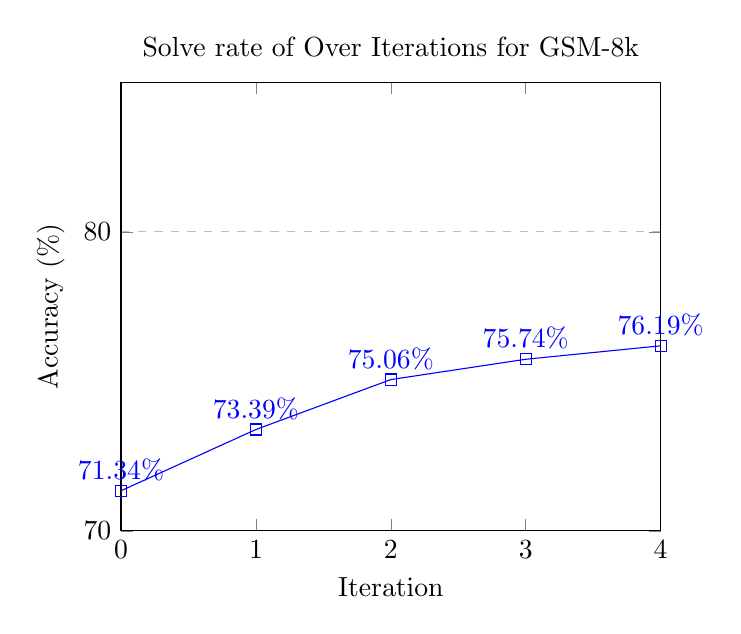
\begin{tikzpicture}
\begin{axis}[
    title={Solve rate of \ours Over Iterations for GSM-8k},
    xlabel={Iteration},
    ylabel={Accuracy (\%)},
    xmin=0, xmax=4,
    ymin=70, ymax=85,
    xtick={0,1,2,3,4},
    ytick={0,10,20,30,40,50,60,70,80,90,100},
    legend pos=north west,
    ymajorgrids=true,
    grid style=dashed,
    nodes near coords,
    point meta=explicit symbolic,
]

\addplot[
    color=blue,
    mark=square,
    ]
    coordinates {
    (0,71.34) [71.34\%]
    (1,73.39) [73.39\%]
    (2,75.06) [75.06\%]
    (3,75.74) [75.74\%]
    (4,76.19) [76.19\%]
    };
\end{axis}
\end{tikzpicture}
    \caption{Improvements in accuracy on the GSM-8k math reasoning benchmark as a function of the \# of iterations of \ours.}
    \label{fig:code_results}
\end{figure}